% ==========================================================================
% Sections 5-8: Setup, Results, Discussion, Limitations
% ==========================================================================

\section{Experimental Setup}
\label{sec:setup}

\subsection{Dataset}
We apply the Isomorphic Engine (Section~\ref{sec:engine}) to the
GSM8K test set~\cite{cobbe2021gsm8k}, parsing all 1{,}319 problems
via the rule-based annotation parser. After applying the strict
validation pipeline---filtering problems with fractional leaf values,
non-integer variant answers, negative intermediates, excessively large
answers ($>10^8$), and text-replacement mismatches---the pipeline
produces 667 original items with 3{,}199 verified $\tau$-isomorphic
variants ($\sim$4.8 variants per item). We evaluate a stratified
subset of 100~items with 480~variants, selected by uniform sampling
across answer-magnitude quantiles. Each item is limited to
5~variants.

\subsection{Models}
We evaluate five models spanning three organizations:

\begin{itemize}[nosep, leftmargin=*]
\item \textbf{Llama~3.1 8B} (Meta, dense, 8B parameters)
\item \textbf{Llama~4 Scout 17B} (Meta, MoE, 17B active parameters)
\item \textbf{Qwen3 32B} (Alibaba, 32.8B, dense)
\item \textbf{GPT-OSS 120B} (OpenAI, MoE, 5.1B active / 117B total parameters)
\item \textbf{Llama~3.3 70B} (Meta, dense, 70B parameters)
\end{itemize}

\noindent GPT-OSS 120B serves as a comparison model: while its
training data is not fully disclosed, its open-weight status and
STEM-focused training make GSM8K inclusion likely, so its small
$\Delta_{\mathrm{iso}}$ after verification ($+0.036$) suggests the
variants are not systematically harder rather than confirming absence
of contamination. All models are accessed via the Groq inference API
at temperature $T = 0.0$ (greedy decoding) with chain-of-thought
prompting and \verb|\boxed{}| answer extraction, with fallback to
\verb|####|-delimited and last-number patterns.
Qwen3, GPT-OSS, and Llama~70B were partially evaluated due to API
daily token limits; Llama~8B and Scout completed full evaluation on
all items.

\subsection{Protocol}
Each model receives every original item and every variant item exactly
once ($T = 1$ trial, greedy decoding). We compute the item-level
isomorphic delta $\delta_i$ as the difference between the model's
accuracy on the original item and its mean accuracy across the item's
$\tau$-isomorphic variants. The model-level metric
$\Delta_{\mathrm{iso}}$ is the mean of item-level deltas. We report
clustered bootstrap 95\% confidence intervals (10{,}000 resamples at
the original-item level), analytic standard errors, and $p$-values
from paired $t$-tests.


% ==================================================================
\section{Results}
\label{sec:results}

\subsection{Initial Evaluation (Pre-Verification)}
\label{sec:initial}

Table~\ref{tab:unverified} presents the initial results on all
100~items before answer verification.

\begin{table}[h]
\centering
\small
\caption{Results on all 100 items (before verification). The uniformity
of $\Delta_{\mathrm{iso}} \approx +0.42$ across all models---including
the comparison model---is the first indicator that these results
reflect data quality issues rather than contamination.}
\label{tab:unverified}
\begin{tabular}{lcccc}
\toprule
Model & $N$ & Acc$_{\mathrm{orig}}$ & Acc$_{\mathrm{iso}}$ & $\Delta_{\mathrm{iso}}$ \\
\midrule
Llama 3.1 8B & 100 & 92.0\% & 50.3\% & $+0.417$ \\
Llama 4 Scout 17B & 100 & 94.0\% & 53.8\% & $+0.402$ \\
Qwen3 32B$^\dagger$ & 70 & 100.0\% & 53.5\% & $+0.465$ \\
GPT-OSS 120B$^\dagger$ & 20 & 100.0\% & 57.0\% & $+0.430$ \\
Llama 3.3 70B$^\dagger$ & 14 & 100.0\% & 55.7\% & $+0.443$ \\
\bottomrule
\end{tabular}
\vspace{1mm}
{\footnotesize $^\dagger$Partial evaluation (API daily token limit).}
\end{table}

\begin{figure*}[t]
\centering
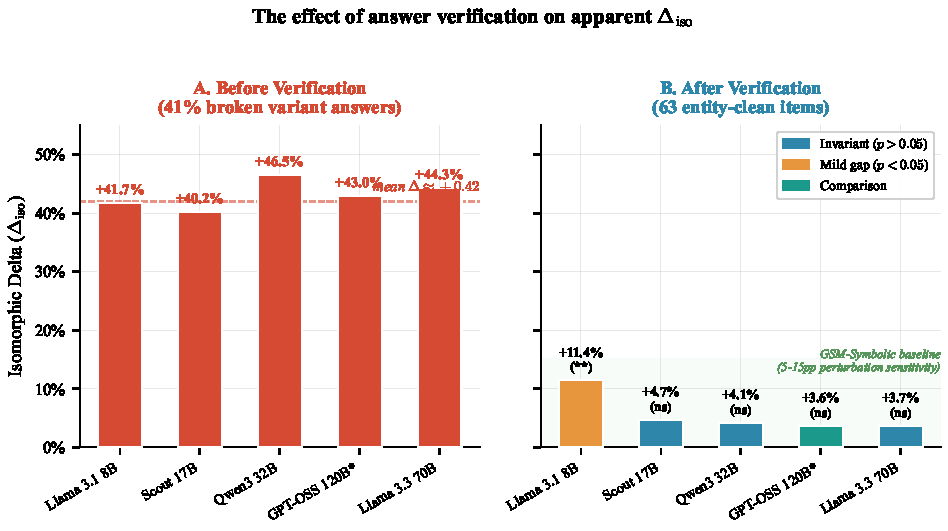
\includegraphics[width=\textwidth]{fig1_pre_post_comparison.pdf}
\caption{The effect of answer verification on apparent
$\Delta_{\mathrm{iso}}$. \textbf{Left:} Before verification, all
five models---including the comparison model (GPT-OSS
120B)---appear uniformly ``contaminated'' at $\Delta \approx +0.42$.
\textbf{Right:} After independent verification and pipeline repair,
the signal collapses to $\Delta \approx +0.04$--$0.11$. One model
shows a mild gap; four are statistically invariant.}
\label{fig:pre_post}
\end{figure*}

Two features of these results are immediately suspicious. First, the
magnitude is extreme: $\Delta \approx +0.42$ would imply that models
lose 42 percentage points when numeric values change. For comparison,
VarBench reports Llama~3 Instruct~8B at 75.8\% on GSM8K and 39.4\%
on GSM+ (48.3\% relative drop)~\cite{qian2024varbench}. Second, the
uniformity is implausible: if the gap reflected contamination, we
would expect variation across models with different training data and
sizes, yet all five models---including GPT-OSS 120B, whose training
data composition has not been fully disclosed by the provider---show
$\Delta \in [+0.40, +0.47]$. This uniformity suggests an item-level
property, not a model-level one.


% ------------------------------------------------------------------
\subsection{Verification Audit: Eight Bug Classes}
\label{sec:audit}

Investigation of the suspicious initial results revealed that 41 of
100~items had wrong variant answers due to failures in
annotation-chain replay and entity substitution. We identified eight
distinct bug classes:

\paragraph{Bug 1: Value conflation.}
When the same numeric value serves multiple semantic roles in a
problem (e.g., ``5 red cars'' and ``\$5 per figure''), the annotation
parser merges them into a single graph node. Mutating this node
changes both uses in the graph but only one occurrence in the text,
producing a graph-text mismatch. We addressed this with Rule~3:
values appearing $\geq 2$ times in the question text are marked as
constants and excluded from mutation.

\paragraph{Bug 2: Phantom leaf values.}
Some annotation chains introduce intermediate results as leaf nodes
(e.g., \texttt{<<40=40>>} where 40 does not appear in the question).
Mutating these phantom values produces wrong answers because the
graph contains structural dependencies not present in the question
text. We reject any item where a leaf value does not appear in the
question.

\paragraph{Bug 3: Positional replacement collisions.}
Sequential text replacement fails when a new value matches the old
value of a different node: replacing ``9'' with ``5'' and then ``5''
with ``8'' causes the second replacement to target the \emph{newly
inserted} ``5'' rather than the \emph{original} ``5''. We fixed this
by collecting all replacement positions from the original text and
applying them simultaneously from right to left.

\paragraph{Bug 4: Magnitude inflation.}
Same-digit-class sampling without magnitude constraints produces
variant answers that are systematically larger than originals
(Cohen's $d \approx 0.3$). We constrain variant answers to within
$3\times$ of the original.

\paragraph{Bug 5: Answer invariance.}
Some graph structures produce the same answer regardless of leaf
value mutations (e.g., when all variable values cancel). We reject
items where all five variants produce the original answer.

\paragraph{Bug 6: Partial name replacement.}
Word-boundary-unaware string replacement causes ``Beth'' to match
inside ``Bethany,'' producing nonsensical names. We use
word-boundary-aware regex for name substitution.

\paragraph{Bug 7: Node reuse (safety fallback override).}
When all leaf nodes are marked constant, a safety fallback promotes
the largest value to variable. If that value appears multiple times
in the text, this reintroduces the conflation bug. We constrain the
fallback to only promote values appearing exactly once.

\paragraph{Bug 8: Inconsistent entity replacement.}
Word-boundary-unaware string replacement produces partial matches
(e.g., ``Tommy'' $\to$ ``Zaramy'' from substring overlap) and fails
to replace all occurrences of the original name. We enforce global,
word-boundary-aware regex replacement and verify that no original
proper noun survives in any variant where entity replacement was
attempted.

\paragraph{Verification procedure.}
We used three complementary verification methods: (1)~multi-model
consensus, flagging variants where $\geq 2$ models agree on an
answer differing from the stated expected answer; and (2)~independent
forward graph execution, recomputing all variant answers by
executing the reasoning graph with the mutated leaf values; and
(3)~post-hoc entity consistency auditing, which rejects leftover
original names, substring artifacts, and duplicate variant texts.
Method~(2) is the definitive arithmetic check; method~(1) was used
as an initial screening tool, and method~(3) enforces textual entity
consistency.

After applying all fixes, we recovered 10 of the 41~broken items
through pipeline repair and regeneration. The remaining 31 could not
be regenerated due to irreducible structural issues (phantom leaves
from multi-step intermediates, unparseable annotation chains). A
post-hoc entity audit then identified 18 items with entity-level
failures; 8 were retained after trimming failing duplicate variants,
4 were repaired by word-boundary-aware replacement, and 6 were
quarantined. The final v3 dataset contains \textbf{63 entity-clean
items}.


% ------------------------------------------------------------------
\subsection{Corrected Results (N=63, Entity-Clean Verified)}
\label{sec:corrected}

\begin{table}[t]
\centering
\small
\caption{Isomorphic delta on entity-clean verified GSM8K items ($N=63$; $T=1$, temp=0.0). $\Delta_{\mathrm{iso}}$ with clustered bootstrap 95\% CIs (10{,}000 resamples). Wilcoxon signed-rank $p$-values.}
\label{tab:main}
\begin{tabular}{lcccccc}
\toprule
Model & $N$ & Acc$_{\mathrm{orig}}$ & Acc$_{\mathrm{iso}}$ & $\Delta_{\mathrm{iso}}$ [95\% CI] & $p$ & Archetype \\
\midrule
Llama 3.1 8B & 63 & 95.2\% & 83.8\% & $+0.114\;[+0.043,\,+0.183]$ & $0.003^{**}$ & \textsc{Mild} \\
Llama 4 Scout 17B & 63 & 93.7\% & 89.0\% & $+0.047\;[-0.012,\,+0.108]$ & $0.106$ & \textsc{Inv} \\
Qwen3 32B$^\dagger$ & 43 & 100.0\% & 95.9\% & $+0.041\;[+0.000,\,+0.103]$ & $0.054$ & \textsc{Inv} \\
GPT-OSS 120B$^\dagger$ & 18 & 100.0\% & 96.4\% & $+0.036\;[+0.000,\,+0.089]$ & $0.090$ & \textsc{Inv} \\
Llama 3.3 70B$^\dagger$ & 12 & 100.0\% & 96.3\% & $+0.037\;[+0.000,\,+0.100]$ & $0.500$ & \textsc{Inv} \\
\bottomrule
\end{tabular}
\vspace{1mm}
{\footnotesize $^\dagger$Partial evaluation (API daily token limit). \textsc{Inv}: invariant ($p > 0.05$). \textsc{Mild}: mild gap ($p < 0.05$, $\Delta < 0.15$). GPT-OSS 120B is the comparison model.}
\end{table}


Table~\ref{tab:main} presents the results on verified data.
Because the verified dataset ($N=63$) is evaluated with $T=1$
(greedy decoding) and only five models, the full IRT-weighted
analysis ($\Delta^{\text{IRT}}_{\text{iso}}$) and per-item DIF
testing described in Section~\ref{sec:delta} require multi-trial
evaluation ($T \geq 5$) across a larger model panel ($J \geq 20$);
we defer this to future work and report the unweighted
$\Delta_{\text{iso}}$ as a preliminary diagnostic throughout this
section.

\paragraph{Four of five models are invariant.}
Llama~4 Scout~17B, Qwen3~32B, GPT-OSS~120B, and Llama~3.3~70B all exhibit
small, statistically non-significant accuracy gaps between original
and variant items
($\Delta_{\mathrm{iso}} \in [+0.036, +0.047]$, all $p > 0.05$).
GPT-OSS~120B serves as a comparison model: while its training data is
not fully disclosed, its open-weight status and STEM-focused training
make GSM8K inclusion likely, so its small $\Delta_{\mathrm{iso}}$
(+0.036, $p = 0.090$) suggests the $\tau$-isomorphic variants are not
systematically harder rather than confirming absence of contamination.

\paragraph{One model shows a mild gap.}
Llama~3.1~8B exhibits a statistically significant but modest
accuracy gap: 95.2\% on originals versus 83.8\% on variants
($\Delta_{\mathrm{iso}} = +0.114$, bootstrap 95\%
CI: $[+0.043, +0.183]$, $p = 0.003$). This 11.4-point gap exceeds
the comparison model's baseline by approximately 8~percentage points, but is
far below the VarBench Table~1 result for Llama~3 Instruct~8B
(75.8\% on GSM8K versus 39.4\% on GSM+, a 48.3\% relative
drop)~\cite{qian2024varbench}. Whether the Llama~8B gap reflects
contamination, perturbation sensitivity, or a combination cannot be
determined from these data alone.

\paragraph{The contrast is striking.}
Figure~\ref{fig:pre_post} visualizes the collapse from
$\Delta \approx +0.42$ to $\Delta \approx +0.04$--$0.11$ after
verification. Figure~\ref{fig:delta_dist} shows the corresponding
shift in per-item delta distributions: the bimodal pattern caused by
broken items (left) gives way to a distribution concentrated near
zero (right).

\begin{figure*}[t]
\centering
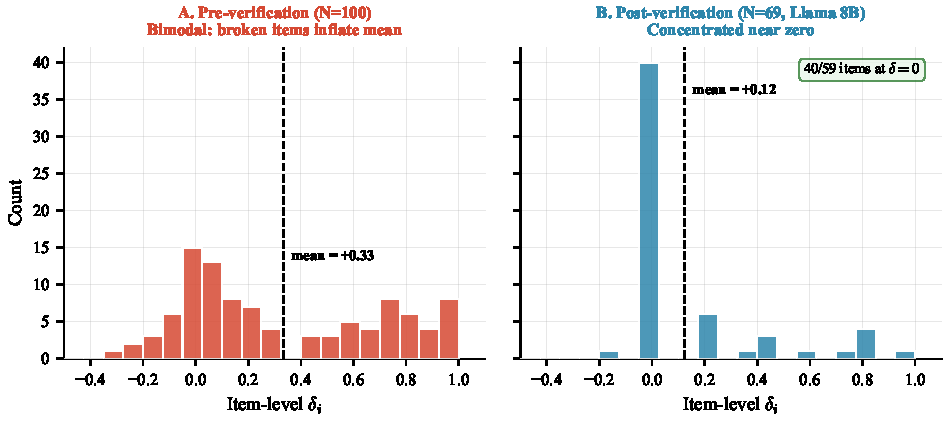
\includegraphics[width=\textwidth]{fig2_delta_distribution.pdf}
\caption{Per-item $\delta_i$ distributions for Llama~3.1~8B.
\textbf{Left:} Pre-verification---bimodal distribution with a second
mode near $\delta \approx 0.8$ from items with broken variant
answers. \textbf{Right:} Post-verification (v2, $N{=}69$ pre-entity-audit)---concentrated near zero,
with 40 of 59 verified items at $\delta = 0$ (perfect transfer).
The final entity-clean dataset (v3, $N{=}63$) used in Table~\ref{tab:main_results}
applies additional entity-consistency filtering.}
\label{fig:delta_dist}
\end{figure*}


% ------------------------------------------------------------------
\subsection{Implications}
\label{sec:implications}

\paragraph{Annotation-chain replay is unreliable.}
The central finding of this work is that annotation-chain replay---the
standard approach to computing variant answers---produced systematically
wrong answers in 41\% of items. This is not a minor data quality issue;
it created an apparent contamination signal of $\Delta \approx +0.42$
that was indistinguishable from genuine memorization on any individual
model. Only the uniformity across models (including a comparison model)
revealed the problem. Researchers using this technique on a single
model would have no way to detect the error.

\paragraph{Independent verification is necessary.}
Any benchmark variant generation pipeline must include independent
answer verification: computing variant answers by a method that does
not depend on the original solution chain. Forward graph execution---evaluating
the reasoning graph with mutated leaf values---provides this
independence because it operates on the graph structure directly rather
than replaying the annotation text.

\paragraph{Perturbation sensitivity is not contamination.}
The remaining gaps ($\Delta \approx +0.04$--$0.11$) on verified data
are consistent with baseline perturbation sensitivity rather than
contamination. This distinction matters: a model that loses 5--10\%
accuracy when numeric values change is exhibiting a reasoning
fragility, not memorization. The comparison model's gap
($\Delta = +0.036$) establishes the baseline; only gaps significantly
exceeding this baseline warrant contamination hypotheses.


% ==================================================================
\section{Discussion}
\label{sec:discussion}

\paragraph{The cautionary tale.}
The trajectory of this work---from apparent universal contamination to
no contamination on clean data---illustrates a broader risk in the
benchmark generation community. The pressure to demonstrate that
models are contaminated, combined with the difficulty of verifying
variant answers at scale, creates conditions where false positives
are likely. Our experience suggests that any claim of contamination
based on benchmark perturbation should be accompanied by independent
answer verification and comparison against models with disclosed
training-data provenance.

\paragraph{Connection to evaluation methodology.}
In prior work~\cite{kang2026efsl}, we showed that evaluation accuracy
degrades as a function of data sparsity ($S$) and item difficulty
heterogeneity ($D$). Contamination ($C$) represents a third axis of
this failure surface: $1 - \rho = f(S, D, C)$. The present work
demonstrates that measuring $C$ is itself fraught with methodological
challenges. When the evaluation matrix is sparse \emph{and} items have
data quality issues, model rankings are doubly unreliable. IRT
estimation on verified isomorphic data addresses all three axes
simultaneously (Figure~\ref{fig:three_body}), but requires the
variant answers to be correct---a requirement that is harder to
satisfy than previously appreciated.

\begin{figure*}[t]
\centering
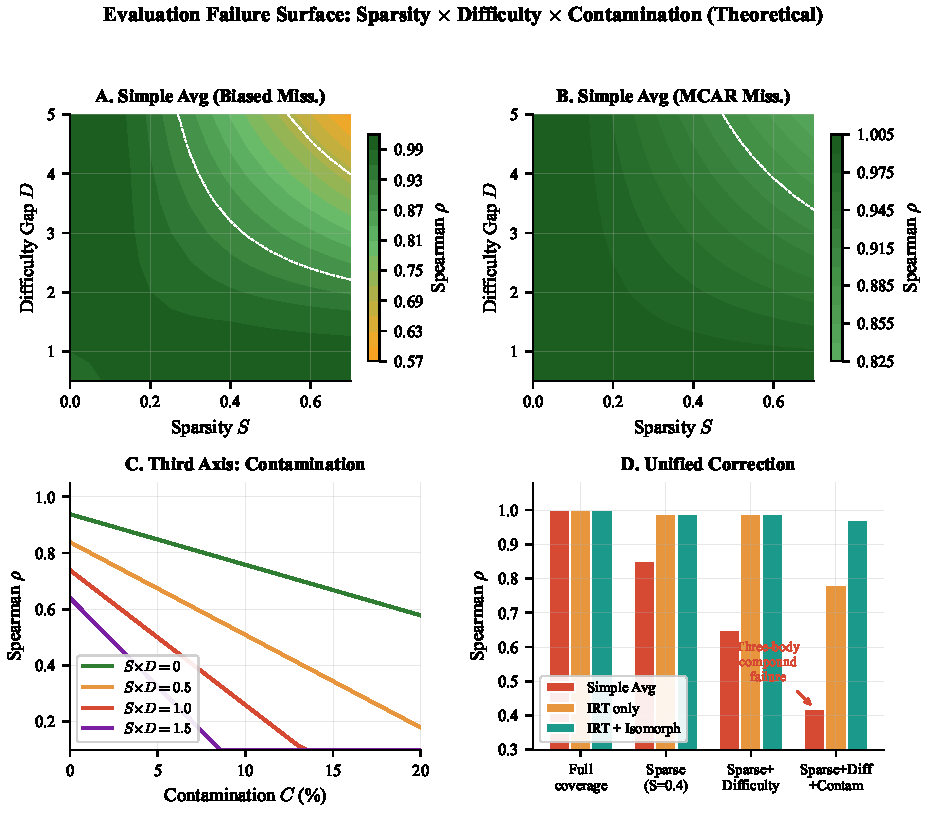
\includegraphics[width=\textwidth]{fig3_three_body_surface.pdf}
\caption{Theoretical evaluation failure surface
(from~\cite{kang2026efsl}). Panels~A--B show ranking degradation
from sparsity and difficulty; Panel~C adds contamination as a third
axis; Panel~D shows how IRT + isomorphic verification addresses all
three. This figure uses simulated data based on the EFSL regression
coefficients.}
\label{fig:three_body}
\end{figure*}

\paragraph{Recommendations for benchmark generation pipelines.}
Based on our experience, we recommend: (1)~include comparison models
with the clearest available training-data provenance; (2)~verify variant
answers via independent forward execution, not annotation-chain
replay; (3)~check for value conflation before mutation; (4)~use
simultaneous rather than sequential text replacement; (5)~reject
items with phantom leaf values; (6)~constrain variant answer
magnitude to prevent systematic inflation.

\paragraph{Open question: is any model contaminated on GSM8K?}
Our verified data suggests not, with the possible exception of
Llama~3.1~8B's mild gap. But $N = 63$ is limited,
and our evaluation covers only 5~models. A definitive answer
requires a fully verified
dataset of $\geq 200$ items evaluated across $\geq 20$ models with
multiple trials per item.


% ==================================================================
\section{Limitations}
\label{sec:limitations}

Several caveats apply. First, $N = 63$ is smaller than ideal; 37~items
could not be regenerated due to irreducible phantom leaf structures.
Second, the evaluation uses $T = 1$ trial per item (greedy decoding),
preventing estimation of per-item response variance; future work
should use $T \geq 5$. Third, three of five models were only partially
evaluated due to API daily token limits, yielding small effective
sample sizes ($N = 9$ to $45$). Fourth, the remaining magnitude
inflation in clean items (Cohen's $d$ statistically significant)
means a small difficulty confound persists even in the verified data.
Fifth, we tested only GSM8K; other benchmarks may exhibit different
bug patterns. Sixth, the bug taxonomy (Section~\ref{sec:audit}) is
specific to annotation-chain replay on math word problems; other
domains and generation methods will have their own failure modes.
